
\subsubsection{Introduction}

In parameterized convection models for planetary thermal evolution the heat transport characteristics 
of the convecting mantle are formulated in a pseudo steady state approximation. 
This is done by parameterization of the surface heatflux as a function of convective vigor, 
through the non-dimensional Nusselt number $\Nunb$. 
$\Nunb$ is usually expressed in terms of the 
Rayleigh number $\Ranb$ as $\Nunb \sim C\, \Ranb^\beta$, where $C$ is a 
constant depending on the domain geometry
(please do read section 1 of Wolstencroft \etal (2009) \cite{wodd09} 
for more information, check also Plumley \& Julien (2019) \cite{plju19} and references therein, 
also Korenaga (2003) \cite{kore03}).

In this lab exercise you will investigate the characteristics of steady-state Rayleigh-Benard convection 
and determine the relation between the Nusselt and Rayleigh number experimentally, 
by means of numerical modelling. In particular you will measure the heatflow through the top surface of 
a 2D model of a convecting layer, as a function of the Rayleigh number, expressed in the temperature 
contrast across the convecting layer. 
This is done by a series of modelling experiments where the coupled equations for thermal convection are solved 
numerically using finite element methods.

The following sections contain descriptions of the numerical model and the experiments to be done. 

%........................................................
\subsubsection{Reminder of the governing model equations}

In this computerlab you will perform experiments with numerical solutions of the 
coupled equations describing thermal convection in an 
incompressible viscous fluid with infinite Prandtl number\footnote{In heat transfer problems, 
the Prandtl number controls the relative thickness of 
the momentum and thermal boundary layers. When Pr is small, it means that the heat diffuses 
quickly compared to the velocity (momentum).}.

In what follows, the assumption is made that geological materials can be treated as fluids (with 
special properties) within the realm of continuum fluid mechanics.
A Boussinesq approximation is applied, neglecting density variations in the equations except 
in the buoyancy term of the momentum conservation equation. We consider two-dimensional problems.

\begin{eqnarray}
{\vec \nabla}\cdot {\bm \sigma} + \rho(T) {\vec g} &=& {\vec 0} \label{eq_moce}\\
{\vec \nabla}\cdot {\vec \upnu} &=& 0 \label{eq_mace}\\
{\bm \sigma} &=& -p {\bm 1} + {\bm \tau} \label{steq}\\
{\bm s} &=& 2 \eta \dot{\bm \varepsilon} \label{stwomu}\\
\dot{\bm \varepsilon}  &=& \frac{1}{2} \left( {\vec \nabla}{\vec \upnu} 
+ ({\vec \nabla}{\vec \upnu})^T  \right) \label{epsdot} \\
\rho_0 C_p \left( \frac{\partial T}{\partial t}  + {\vec \upnu}\cdot {\vec \nabla} T\right) 
&=& {\vec \nabla}\cdot (k {\vec \nabla}T)  \label{eqhte} \\
\rho(T) &=& \rho_0 (1 - \alpha (T-T_0)) 
\end{eqnarray}

Equation (\ref{eq_moce}) is the momentum conservation equation and 
Eq. (\ref{eq_mace}) is the mass conservation equation for incompressible fluids.
One can resolve the stress tensor ${\bm \sigma}$ into its spherical part $-p{\bm 1}$ and 
its stress deviation ${\bm \tau}$ (see Eq. (\ref{steq})), where the deviatoric stress tensor is 
proportional to the strain rate tensor $\dot{\bm \varepsilon}$ (see Eq.(\ref{stwomu})) through the 
dynamic viscosity $\eta$. 
Finally Eq. (\ref{epsdot}) relates the strain rate tensor to the velocity field.

Equations (\ref{eq_moce}), (\ref{eq_mace}), (\ref{steq}), (\ref{stwomu}) and (\ref{epsdot}) all 
together lead to the following form of the Stokes equations:
\begin{eqnarray}
{\vec \nabla}\cdot [\eta ({\vec\nabla} {\vec \upnu} + {\vec \nabla} {\vec \upnu}^T ) ] 
- {\vec \nabla}p + \rho {\vec g} &=& {\vec 0} \label{mce2} \\
{\vec \nabla}\cdot {\vec \upnu} &=& 0 \label{eq_mace2}
\end{eqnarray}
Equation (\ref{mce2}) is an elliptic equation characterized by the 
fact that changes in buoyancy and constitutive relationships {\it anywhere} 
in the domain have an immediate influence on the entire domain.

\begin{center}
\begin{tabular}{ll}
\hline
symbol & meaning and dimension \\
\hline
\hline
${\vec g}$ & gravity acceleration vector (\si{\metre\per\square\second}) \\
$L_x$, $L_y$ & domain size (\si{\metre}) \\
$p$ & pressure  (\si{\pascal}) \\
${\bm \tau}$ & deviatoric stress vector  (\si{\pascal}) \\
${\vec \upnu}=(u,v,w)$ & velocity (\si{\metre\per\second}) \\
$\dot{\bm \varepsilon}$ & strain-rate tensor (\si{\per\second}) \\
$\eta$ & viscosity (\si{\pascal\second})\\
$\rho,\rho_0$ & mass density (\si{\kg\per\cubic\metre}) \\
${\bm \sigma}$ & stress tensor  (\si{\pascal})  \\
$k$ & heat conductivity (\si{\watt\per\meter\per\kelvin}) \\
$C_p$ & heat capacity (\si{\joule\per\kelvin})\\
$\alpha$ & thermal expansion (\si{\per\kelvin}) \\
\hline
\end{tabular}\\
{\captionfont Nomenclature}
\end{center}


%........................................................
\subsubsection{Numerical solution of the equations}

Introduced in the late 1950s, the finite element method (FEM) \cite{hugh,zita1,zita2,zita3} 
has emerged as one of the most powerful numerical methods so far devised. 

A thorough mathematical treatment of the finite element formulation of the equations gouverning the physics of the system is beyond the scope of this 
computer practical, and has been exposed rigorously in Section~\ref{solvingFEM} 
and in various textbooks such as \cite{dohu03} or \cite{gunz89}.

We wish to study the system at steady state, which means that it no more changes in time. 
In practice, only he heat transport equation contains a time (derivative) term so we actually wish 
to solve these three (coupled) equations:

\begin{eqnarray}
{\vec \nabla}\cdot [\eta ({\vec\nabla} {\color{red}{\vec \upnu}} 
+ {\vec \nabla} {\color{red}{\vec \upnu}}^T ) ] 
- {\vec \nabla}p + \rho({\color{blue}T}) {\vec g} &=& {\vec 0}   \\
{\vec \nabla}\cdot {\color{red} {\vec \upnu}} &=& 0 \\
\rho_0 C_p {\color{red} {\vec \upnu}}\cdot {\vec \nabla} {\color{blue}T} &=& k \Delta {\color{blue}T} 
\end{eqnarray} 

The main problem is clearly visible in the third one: with respect to the velocity and 
temperature unknowns this is a nonlinear equation! 
We therefore have to design a strategy (an algorithm) which will allow us to solve these 
equations. 

One simple approach is as follows: the equations are not solved in a coupled manner. 
The obtention of a new set of variables $({\bm v},p,T)$ is the product of a two-stage process:
\begin{enumerate}
\item assume temperature known, solve for velocity (and pressure) field (the first two equations)
\item assume velocity known, solve for temperature (the last equation).
\end{enumerate}

These two steps need to be repeated as long as the system has not converged to a steady solution. 
The code therefore implements iterations and these iterations stop when either the maximum number 
of iterations nstep is reached or convergence has been reached (i.e. temperature does not change 
substantially between two consecutive iterations). The structure of the code 
is then as follows:

\begin{flushright} {\tiny {\color{gray} (tikz\_md1416.tex)}} \end{flushright}
%~~~~~~~~~~~~~~~~~~~~~~~~~~~~~~~~~~~~~~~~~~~~~~~~~~~~~~~~~~~~~~~~~~~~~~~~~~~~~~~~~~~~~~~~~~~~~~~~~~


\begin{center}
\begin{tikzpicture}
%\draw[step=0.5cm,gray,very thin] (0,0) grid (7,10); %background grid

\draw[blue, thick] (2.,0.5) rectangle (6,1.5);
\draw[blue, thick] (2.,4.5) rectangle (6,5.5);
\draw[blue, thick] (2.,6.5) rectangle (6,7.5);
\draw[blue, thick] (2.,9)   rectangle (6,10);

\draw[>=triangle 45, line width=0.3mm, ->] (2.5,3)--(1,3)--(1,8.5)--(4,8.5) ;   

\draw[>=triangle 45, line width=0.3mm, ->] (4,9)--(4,7.5) ;   
\draw[>=triangle 45, line width=0.3mm, ->] (4,6.5)--(4,5.5) ;   
\draw[>=triangle 45, line width=0.3mm, ->] (4,4.5)--(4,3.5) ;   
\draw[>=triangle 45, line width=0.3mm, ->] (4,2.5)--(4,1.5) ;   

\draw[thick] (2.5,3)--(4,2.5)--(5.5,3)--(4,3.5)--cycle;

\node[] at (4,9.5) {\small Initial Temperature};
\node[] at (4,7) {\small Solve Stokes Eqs.};
\node[] at (4,5) {\small Solve energy Eq.};
\node[] at (4,3) {\small convergence?};
\node[] at (4,1) {\small Export data};

\node[] at (4.2,2.2) {\small Y};
\node[] at (2.2,3.2) {\small N};

\node[] at (4.5,6) {$\vec{\upnu},p$};
\node[] at (4.5,4) {$T$};

\end{tikzpicture}
\end{center}






%%%%%%%%%%%%%%%%%%%%%%%%%%%%%%%%%%%%%%%%%%%%%%%%%%
\subsubsection{Two-dimensional convection in a unit box}

This benchmark deals with the 2-D thermal convection of a fluid 
of infinite Prandtl number in a rectangular closed cell.
In what follows, we will focus on the case 1a, 1b, and 1c experiments as shown in \cite{blbc89}:
steady convection with constant viscosity in a square box.

The temperature is fixed to zero on top and to $\Delta T$ at the bottom, 
with reflecting symmetry at the sidewalls (i.e. $\partial_x T=0$) 
and there are no internal heat sources. 
Free-slip conditions are implemented on all boundaries. 

The Rayleigh number is given by
\begin{equation}
\Ranb = \frac{\alpha g_y \rho_0 \Delta T h^3 }{\kappa \nu}
=\frac{\alpha g_y \Delta T h^3 \rho^2 C_p}{k \eta}
\end{equation}

In what follows, I use the following parameter values:  
$L_x=L_y=1$, $\rho_0=C_P=k=\eta=1$, $T_0=0$, $\alpha=10^{-4}$, $g=10^{4}\Ranb$.
%and I run the model with $Ra=10^4,10^{5}$ and $10^6$.

The initial temperature field is given by 
\begin{equation}
T(x,y)=(1-y) - 0.01\cos(\pi x/L_x) \sin(\pi y/L_y)
\end{equation}
The perturbation in the initial temperature fields leads to 
a perturbation of the density field and sets the fluid in motion. 
Depending on the initial Rayleigh number, the system ultimately reaches a 
steady state after some time. 
%The steady-state 
%temperature fields of case 1a,b,c are shown in Fig. \ref{fig_blankenbach1}.

The root mean square of the velocity field in the whole domain is defined as 
follows:
\begin{equation}
\upnu_{rms}
= \left( \frac{1}{V_\Omega} \int_\Omega |{\vec \upnu}|^2 \; dV \right)^{1/2} 
= \left( \frac{1}{L_xL_y} \int_\Omega (u^2+v^2) \; dV \right)^{1/2} 
\label{eq_vrms}
\end{equation}

%was measured for a $100\times100$ grid resolution for all three cases
%and divided by the corresponding steady state values presented in \cite{blbc89}. 
%Results are shown in Fig. \ref{fig_blankenbach2} and one 
%sees that there is a very good agreement as all three curves ultimately 
%converge to the expected value 1.

The Nusselt number (i.e. the mean surface temperature gradient over mean bottom temperature)
is computed as follows \cite{blbc89}:
\begin{equation}
\Nunb = L_y \frac{\int_0^{L_x} \frac{\partial T}{\partial y}(y=L_y) dx  }{\int_0^{L_x} T(y=0) dx}
\label{eqNu}
\end{equation}
Note that in our case the denominator is equal to $L_x$ since the temperature at the 
bottom is prescribed to be 1.

%The case 1a results are shown in Fig. \ref{fig_blankenbach3} for three grid resolutions.  
%We see that the Nusselt number converges towards the expected value and that with 
%increasing resolution the error decreases. 
%The relative error on the Nusselt number has been measured for 
%various grid resolutions with $Ra=10^4$ and %is shown in Fig. (\ref{fig_blankenbach4}).
%was found to decrease quadratically with the element size.

Finally, the steady state root mean square velocity and Nusselt number measurements
are indicated in the followiug table alongside those of Blankenbach \etal \cite{blbc89} 
and Tackley \cite{tack94}.
(Note that this benchmark was also carried out and published in 
other publications \cite{trha98,albe00,gery10,dawk11,lezh11} but since they did not provide  a complete set 
of measurement values, they are not included in the table.)

\begin{center} 
\begin{tabular}{llcc}
\hline
          &           & Blankenbach \etal \cite{blbc89} & Tackley \cite{tack94}    \\
\hline
\hline
$\Ranb=10^4$ & $\upnu_{rms}$ &  $42.864947  \pm 0.000020$ & 42.775 \\
             & $\Nunb$       &  $4.884409   \pm 0.000010$ & 4.878  \\
$\Ranb=10^5$ & $\upnu_{rms}$ &  $193.21454  \pm 0.00010 $ & 193.11 \\
             & $\Nunb$       &  $10.534095  \pm 0.000010$ & 10.531 \\
$\Ranb=10^6$ & $\upnu_{rms}$ &  $833.98977  \pm 0.00020 $ & 833.55 \\
             & $\Nunb$       &  $21.972465  \pm 0.000020$ & 21.998 \\
\hline
\end{tabular}\\ 
{\captionfont Steady state Nusselt number $\Nunb$ and $\upnu_{rms}$ measurements 
as reported in the literature.} 
\end{center} 



%\begin{figure}
%\centering
%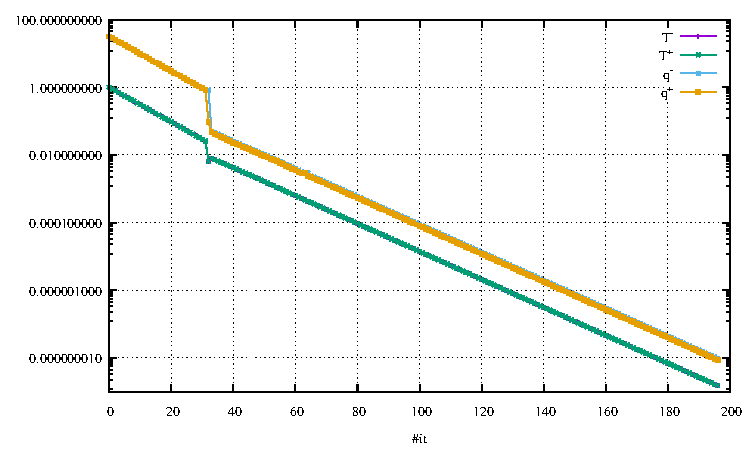
\includegraphics[width=8cm]{blankenbach/convergence.pdf}
%\caption{Steady state Nusselt number as a function of the element size. \label{fig_blankenbach4}}
%\end{figure}

%%%%%%%%%%%%%%%%%%%%%%%%%%%%%%%%%%%%%%%
\subsubsection{Obtaining the python code}

The code is to be downloaded as follows in a terminal:
{\small
\begin{verbatim}
wget https://raw.githubusercontent.com/cedrict/fieldstone/master/python_codes/md/stone.py
\end{verbatim}
}
If you do not know what a terminal is or if you are using Windows, simply copy 
{\small
\begin{verbatim}
https://raw.githubusercontent.com/cedrict/fieldstone/master/python_codes/md/stone.py
\end{verbatim}
}
in the address bar of your web browser, select all, paste it in a file on your computer which 
you save as {\tt stone.py}.

You can run the code in a terminal, in Anaconda, Spyder, etc ... 

%%%%%%%%%%%%%%%%%%%%%%%%%%%%%%%%%%%%%%%
\subsubsection{Experiments}

To conduct the exercise you can change the following parameters (and run the code until convergence):
\begin{itemize}
\item {\tt Lx}: horizontal extent of the domain
\item {\tt Ra}: the Rayleigh number $\Ranb$
\item {\tt tol\_ss}: the steady state detection tolerance
\item {\tt nelx,nely}: the number of elements in $x$ and $y$ directions 
\item {\tt nstep}: the maximum number of iterations to reach steady state
\item {\tt top\_bc\_noslip}: flag to switch no slip boundary conditions at top boundary (default is free slip)
\item {\tt bot\_bc\_noslip}: flag to switch no slip boundary conditions at 
      bottom boundary (default is free slip)
\end{itemize}

Results are written out to {\sl .ascii} files and to {\sl .vtu} files. You can produce 
plots with python (matplotlib), gnuplot or even excel, as long as these are not pixelated in your report, 
that they are labeled, captioned, and their axes too.  
Have a thorough look at the code, read {\bf all} instructions, and carry out the following tasks:

\begin{itemize}
\item Determine the Nusselt number at steady state for a range of Rayleigh numbers, 
starting from a subcritical value. 
Produce a plot of $\Nunb$ against $\Ranb$ using double logarithmic axes. 
Determine the critical Rayleigh number. 

\item The code produces data files containing `snapshots' of the resulting numerical solution 
of the temperature and velocity fields in a suitable format ({\tt .vtu}) for visualization with 
graphics program {\sl paraview}. 
Produce colorplots with paraview of the temperature field, for three contrasting Rayleigh number cases, 
and discuss them.

\item Determine the logarithmic slope or powerlaw index $\beta$ defined in the introduction.

\item Produce such a curve for various grid resolutions. How can you explain the differences in 
the results ? Produce a plot of $\Nunb$ as a function of the grid spacing. 

\item Look at how the $\upnu_{rms}$ values at steady state depend on $\Ranb$. 

\item For three contrasting $\Ranb$ values, plot the temperature profiles 
(data to be found in {\sl T\_profile.ascii}) on a single plot and discuss the obtained figure.

\item Set the number of points in the horizontal directions to 16. Choose $\Ranb=10^5$ 
and progressively increase the number 
of points in the vertical direction. Report on the variation of the $\Nunb$ number at steady 
state as a function of the vertical resolution.

\item Estimate the value of the critical Rayleigh number from your Nusselt number plot and 
investigate the difference with the value found in Rayleigh's linear stability analysis 
for a layer of depth $h$ and infinite horizontal extent, $\Ranb_C = (27/4)  \pi^4$ 
(see Section~\ref{ss:sarb}).

\item Change the initial temperature profile to something more random, repeat some of these experiments. 
What can you conclude ?

\item change the top and bottom boundary conditions from free-slip to no-slip. How 
does this influence $\Ranb_c$ ?

\item Bonus: Explore the effect of the aspect ratio of the domain on $\Ranb_c$ and the slope $\beta$.

\item Bonus: change the viscosity function so that the viscosity is 1 in the lower half of the domain 
and $10^m$ in the upper half with $m>1$. Explore \& discuss ...

\end{itemize}


\vspace{2cm}

Relevant sources:
\begin{itemize}
\item Chapter \ref{chapt3} presents the physical equations in more detail. 
\item Stone 88 shows examples of mantle-scale convection.
\item \url{https://youtu.be/YIN9Dcq31x0}
\item \url{https://youtu.be/5SPCU1sFGGc}
\item \url{https://youtu.be/ln7QBN0IRTs}
\item \url{https://youtu.be/d4AS1FmdarU}
\end{itemize} 


